\section{Multirate Signal Processing}
\label{Chap:Multirate}
\begin{frame}[t]{Chapter \autoref{Chap:Multirate}}
\tableofcontents[sections= \value{section}]
\end{frame}


\subsection{Introduction and Motivation}
\begin{frame}[t,allowframebreaks]{Introduction to Multirate Signal Processing}

\begin{itemize}

\item Multirate Signal processing: the field of signal processing which have \textcolor{red}{several sampling rate exist in the system} \cite{DSP_DimitrisManolakis}

\item The changing in sampling rate occurs much often in real world systems

    \begin{itemize}
        \item For example, we have a system A expect data at a sampling rate 10 KHz
        
        \item Another system B expect data at a sampling rate 12 KHz
        
        \item How can I make the 2 systems talk to each other?
        
    \end{itemize}

\end{itemize}


\end{frame}



\subsection{Reminder: Sampling and Notation}
\begin{frame}[t,allowframebreaks]{Reminder about Original Sampling and Notation}


\begin{figure}[ht]
\centering
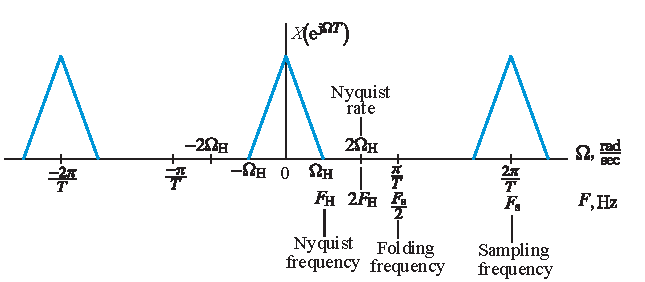
\includegraphics[scale=0.9]{Figures/Sampling/Impulse_Sampling_Terminology}
\caption{Replicated Amplitude Spectrum: Frequency axis in $F$[Hz] and $\omega_c$[rad/s] \cite{DSP_DimitrisManolakis}}
\label{fig:Sampling:Impulse_Sampling_Terminology}
\end{figure}

\begin{itemize}

\item Recall that when sampling in time, images are created at multiple of $F_s$ in CTFT domain along with a scaling factor $\displaystyle\frac{1}{T_s}$


\item This effect will be compared to the effect done by downsampling and upsampling operation to our spectrum

	\begin{itemize}
	\item In other words, we will compare the spectrum after doing down(up)sampling to the spectrum of $X_\delta(\omega_c)$
	\end{itemize}

\item \underline{Notation:} Because now we have some new sampling rate as we will see later, we adopt the following notation for the sampling rate:

	\begin{itemize}
	\item When doing normal Nyquiste sampling $\leftrightarrow \, T_{s_{\text{original}}}$
	
	\item Downsampling $ \leftrightarrow \, T_{\text{downsample}}$
	
	\item Upsampling $ \leftrightarrow \, T_{\text{upsample}}$
	\end{itemize}

\end{itemize}

\end{frame}


\subsection{Downsampling}
\begin{frame}[t,allowframebreaks]{Downsampling Operation}

\begin{figure}[ht]
\centering
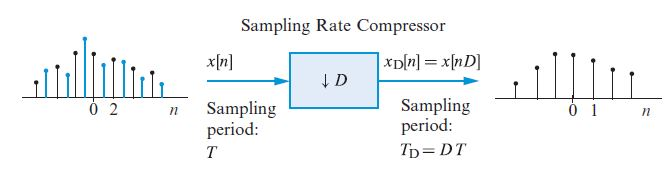
\includegraphics[width = 0.7\textwidth]{Figures/Multirate/dowsampling_block_diagram}
\caption{Block diagram representation of sampling rate compressor system \cite{DSP_DimitrisManolakis}}
\label{fig:Multirate:dowsampling_block_diagram}
\end{figure}

\begin{itemize} 

\item Dowsampling: throwing away samples

\item Vocabulary: downsampler = sampling rate compressor

\item The operation is \textcolor{red} {in the discrete time domain} $x[k]$

\item What happens when we do dowsampling?

	\begin{itemize}
	\item The answer is in the amplitude spectrum 
	\end{itemize}


\end{itemize}
\end{frame}



\begin{frame}[t,allowframebreaks]{Dowsampling Effect on CTFT Amplitude Spectrum}

\begin{itemize}
\item First let's examine relation in the \textcolor{red}{continuous time frequency spectrum}

	\begin{itemize}
	\item Math governing \cite{DSP_DimitrisManolakis}
	
	\end{itemize}

	\begin{equation}
	\begin{array}{rcl}
		X_{\text{decimated}}(\omega_c) \, &=& \, \displaystyle	\frac{1}{T_{\text{downsample}}} \, \displaystyle\sum_{i \, = \, -\infty}^{\infty} X \left(\,  \omega_c \, - \, i \, \omega_{\text{downsample}} \,\right) \\ \\
		&=& \, \displaystyle\frac{1}{T_{s_{\text{original}}} \, D} \, \displaystyle\sum_{i \, = \, -\infty}^{\infty} X \left(\, \omega_c \, - \, \displaystyle\frac{2 \pi}{T_s \, D} \, i \,\right)
\end{array}
\label{Eq:Multirate:Decimation_spectrum_ctft}	
	\end{equation}		

where $\begin{cases}
T_{\text{downsample}} \, = \, D \, \times \, T_{s_{\text{original}}}\\
\omega_{\text{downsample}} \, = \, \displaystyle\frac{2 \pi}{D} \, = \,\displaystyle\frac{\omega_{s_{\text{original}}}}{D} \\
D \, \in \mathbb{N}
\end{cases}$

\begin{figure}[ht]
\centering
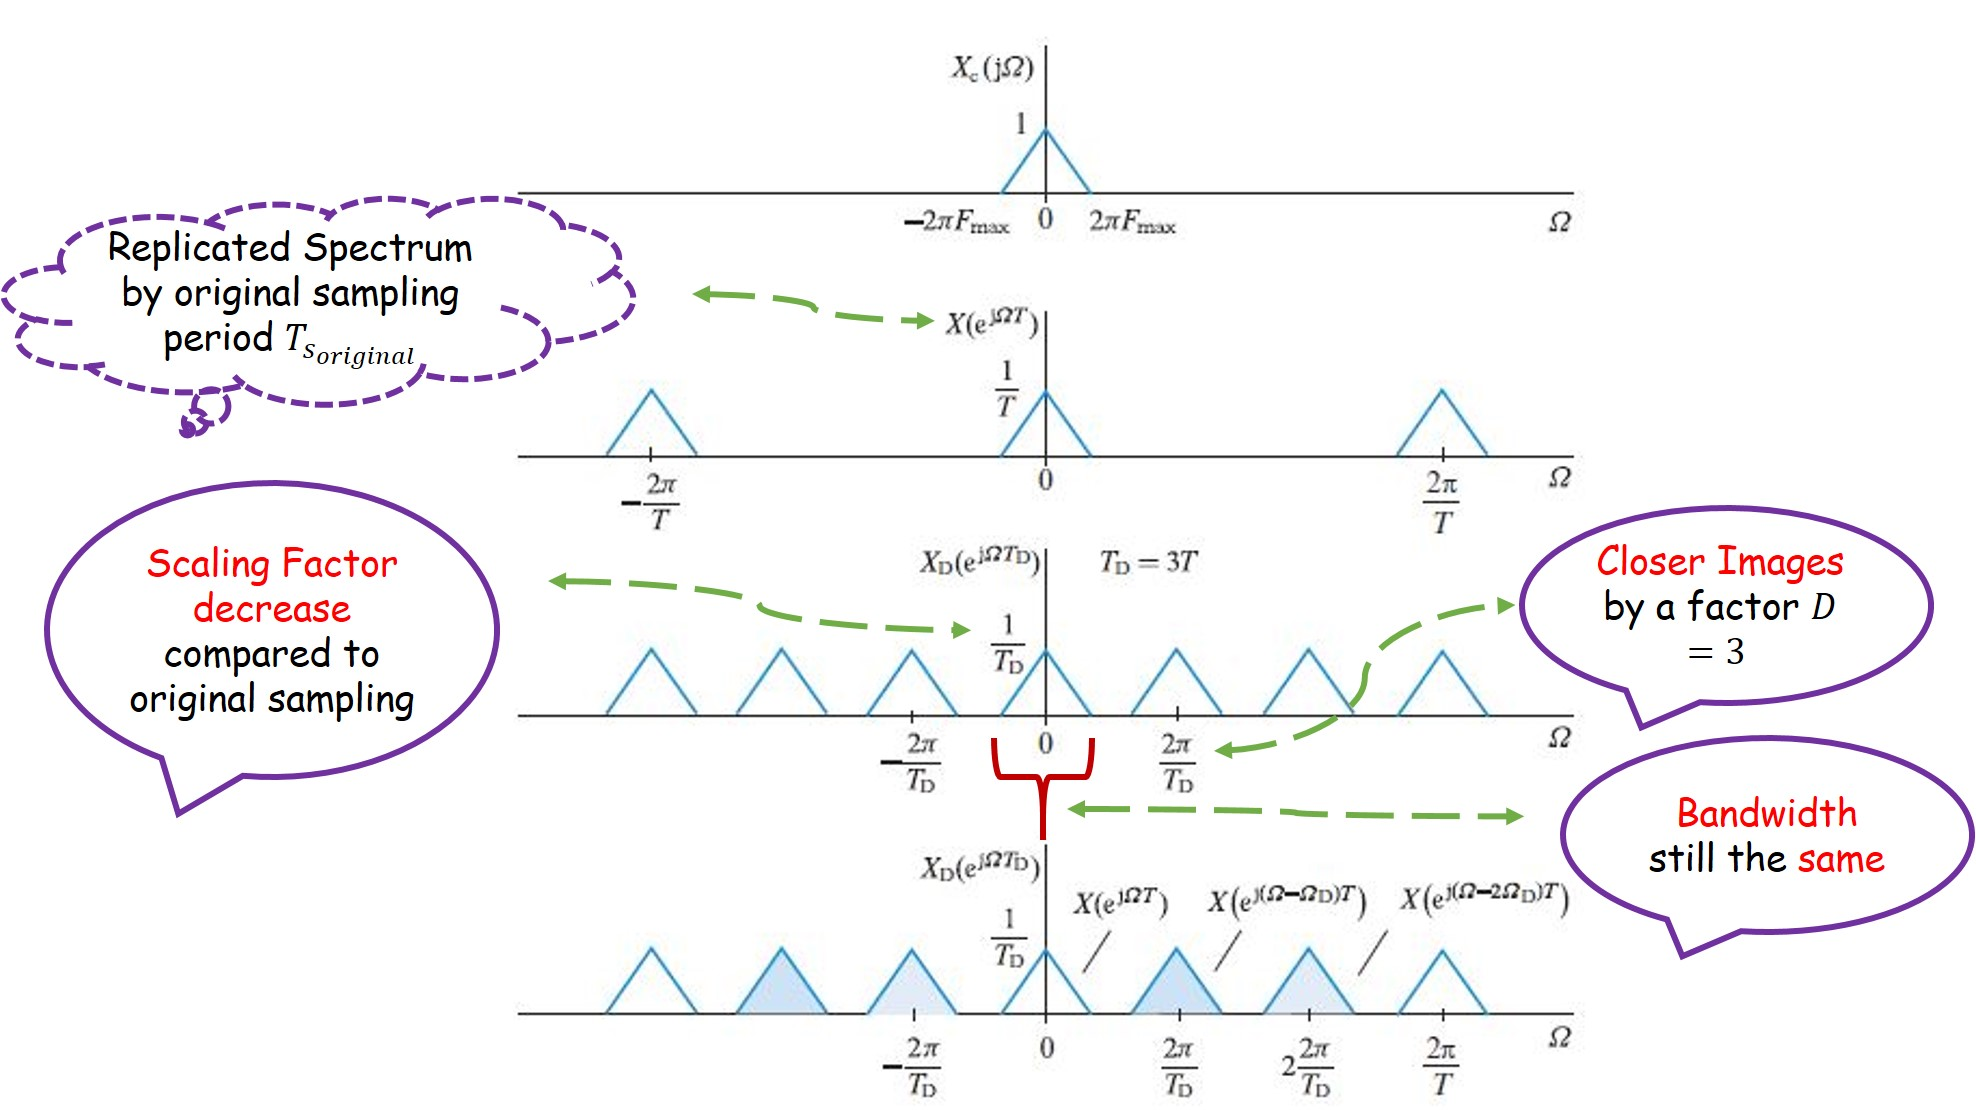
\includegraphics[width = 0.7\textwidth]{Figures/Multirate/dowsampling_ctft_summary}
\caption{Graphical Illustration for equation (\autoref{Eq:Multirate:Decimation_spectrum_ctft}) for CTFT spectrum \cite{DSP_DimitrisManolakis}}
\label{fig:Multirate:dowsampling_ctft}
\end{figure}


\newpage
\item Also keep in mind that we could avoid aliasing by respecting the Nyquiste rate for downsampling

	\begin{itemize}
	\item $\omega_{\text{downsample}} \, = \, \displaystyle\frac{2 \pi}{T_{\text{downsample}}} \, > \, 2 \, \omega_{\text{max}}$
	\end{itemize}

\end{itemize}

\end{frame}



\begin{frame}[t,allowframebreaks]{Dowsampling Effect on DTFT Amplitude Spectrum}

\begin{itemize}
\item Relation between $X_{\text{DTFT}}(\omega_d) $ and $X_{\text{decimated}}(\omega_d) $ 
	
	
	\begin{equation}
	\begin{array}{rcl}
		X_{\text{decimated}}(\omega_d) \, = \, \displaystyle	\frac{1}{D} \, \displaystyle\sum_{i \, = \, 0}^{D \, - \, 1} X_{\text{DTFT}} \left(\,  \displaystyle\frac{\omega_d}{D} \, - \, \displaystyle\frac{2 \pi}{D} \, i \,\right)   
	\end{array}	\label{Eq:Multirate_Sampling_Decimation_spectrum_dtft_relation}
	\end{equation}		
	
	\begin{itemize}
			
	\item A \textcolor{red}{Surprise!}: equation (\ref{Eq:Multirate_Sampling_Decimation_spectrum_dtft_relation}) tells us that our \textcolor{red}{bandwidth will expand (stretch)} by a factor of $D$.

	\end{itemize}


\newpage
\item Some graphical illustrations:


\begin{figure}[ht]
\centering
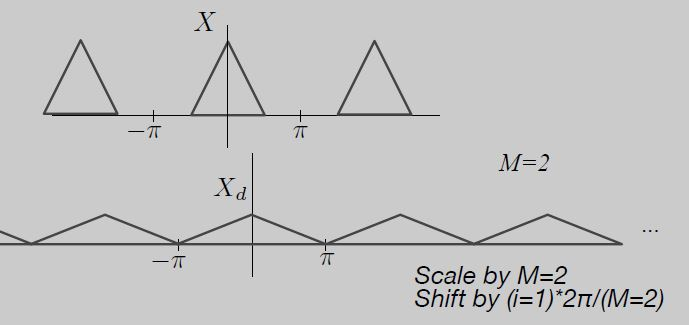
\includegraphics[width = 0.7\textwidth]{Figures/Multirate/dowsampling_example_m_2}
\caption{Downsampling by a factor $D \, = \, 2$}
\label{fig:Multirate:dowsampling_example_m_2}
\end{figure}


	\begin{itemize}
	\item Stretching in the bandwidth
	
	\item Dowsampling $\rightarrow F_s$ decrease $\rightarrow$ replicate will be more closer together
	
	\end{itemize}

\end{itemize}
\end{frame}


\begin{frame}[t,allowframebreaks]{More Dowsampling}



\begin{itemize}


\item Let's downsample more: \textcolor{red}{aliasing occurs !}
	
\begin{figure}[ht]
\centering
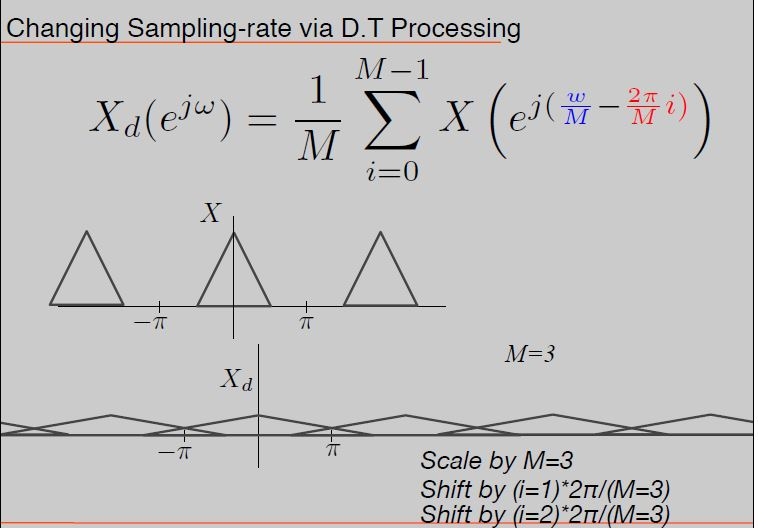
\includegraphics[width = 0.7\textwidth]{Figures/Multirate/dowsampling_example_m_3}
\caption{Downsampling by a factor $M \, = \, 3$ Aliasing occur}
\label{fig:Multirate:dowsampling_example_m_3}
\end{figure}

\newpage
	\item Solution: put an anti-alias filter but in the discrete domain
	
\begin{figure}[ht]
\centering
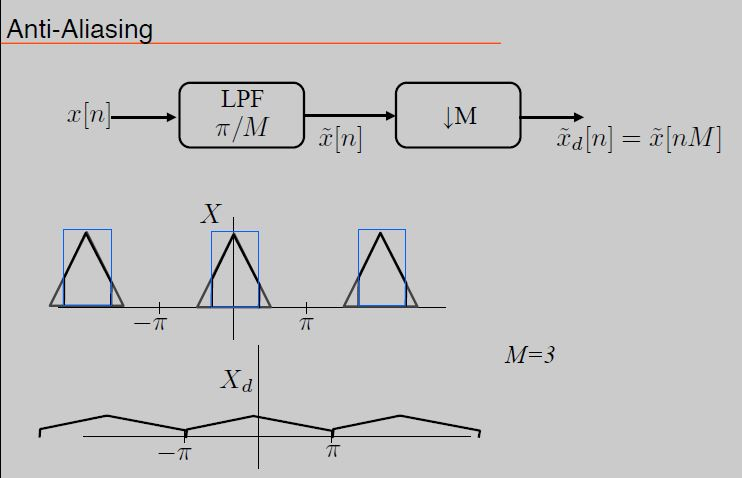
\includegraphics[width = 0.6\textwidth]{Figures/Multirate/dowsampling_antialias_filter}
\caption{Antialias filter then dowsample because downsample can't afford to represent high frequency components}
\label{fig:Multirate:dowsampling_example_m_3}
\end{figure}	
	
		\begin{itemize}
		\item Anti-imaging design choice: $\omega_{\text{cut-off}} \, = \, \displaystyle\frac{\pi}{D}$
		\end{itemize}



\end{itemize}

\end{frame}


\subsection{Upsampling}
\begin{frame}[t,allowframebreaks]{Upsampling Introduction}

\begin{itemize}

\item Very much like to digital-to-analog converter

	\begin{itemize}
	\item Not the same, but they have similarities
	\end{itemize}

\item Recall our ideal digital-to-analog process:

	\begin{itemize}
	\item $x[n] \, = \, x_{\delta}(t) \, \rightarrow \, x_{\text{interpolated}}(t)$, where we have done interpolation using a sinc
	\end{itemize}

\end{itemize}

\end{frame}


\begin{frame}[t,allowframebreaks]{Upsamling Implementation}


\begin{itemize}


\item To implement upsampling, we will do the same thing as in DAC \textcolor{red}{but in the discrete domain}

	\begin{enumerate}	

	\item Start from $x[n]$
	
	\item Expanding by placing 0 between adjacent samples, this will give us $x_{\text{expanded}}[n]$

	\begin{equation}
	x_{\text{expanded}}[n] \, = \, \begin{cases}
	x\left[\, \displaystyle\frac{n}{L} \,\right] \quad n \, =\, 0 \, ; \, \pm L \, ; \, \pm 2L \, \cdots \\
	0 \quad \text{otherwise}
	\end{cases}
	\label{Eq:Multirate:Exapanding}
\end{equation}		

\begin{figure}[ht]
\centering
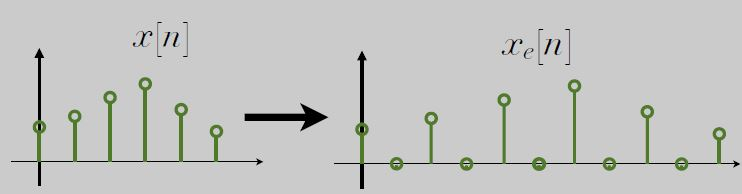
\includegraphics[width = 0.6\textwidth]{Figures/Multirate/upsampling_expansion}
\caption{Expansion in the discrete time domain}
\label{fig:Multirate:upsampling_expansion}
\end{figure}
	
	\begin{itemize}
	\item The expansion of equation (\ref{Eq:Multirate:Exapanding}) also can be viewed as a convolution between the orignal discrete time signal $x[n]$ and a \textcolor{red}{shifted discrete delta}
	
	\begin{equation}
	x_{\text{expanded}}[n] \, = \, \displaystyle\sum\limits_{i \, = \, - \infty}^{\infty} x[i] \, \times \,  \delta[n \, - \,  i \, L]
\end{equation}		
	
\end{itemize}		
	
	\item Interpolation of the expanded signal using a \textcolor{red}{discrete time} sinc 
	
		\begin{itemize}
		\item Be aware that this is a \textcolor{red}{bandlimited interpolation}
		\end{itemize}
	
\begin{figure}[ht]
\centering
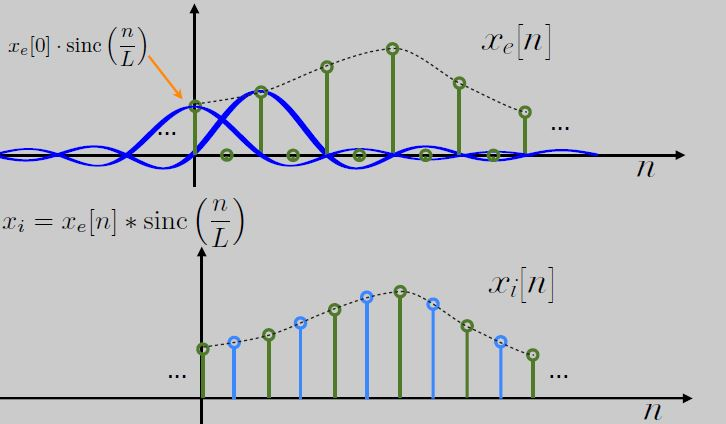
\includegraphics[width = 0.6\textwidth]{Figures/Multirate/upsampling_convolution}
\caption{Convolving the expanded signal with discrete time sinc (bandlimited interpolation)}
\label{fig:Multirate:upsampling_convolution}
\end{figure}


	
 \end{enumerate}

 
\end{itemize}

\end{frame}


\begin{frame}[t,allowframebreaks]{Upsampling Effect on DTFT spectrum}

\begin{itemize}

\item Upsampling \textcolor{red}{compress the DTFT spectrum} by a factor of $L$ \textcolor{cyan}{and} \textcolor{red}{ create replications (Images) also}

\begin{itemize}

\item This is expected since upsampling is like resampling , and we already know that sampling creates images of a spectrum
\end{itemize}

\item \underline{Proof:}

\begin{enumerate}

\item Begin with DTFT definition for the expanded signal $x_{\text{expanded}}[k]$

\begin{equation}
X_{\text{expanded}}(\omega_d)  =  \displaystyle\sum\limits_{k \, = \, - \infty}^{+\infty} x_{\text{expanded}}[k] \, e^{-j \, \omega_d \, k} 
\end{equation}


\item However, we note from equation (\autoref{Eq:Multirate:Exapanding}) that $x_{\text{expanded}}[k]$ exist only for multiple of $L$, the upsampling factor which means that we can change the limit of summation and sum up only for $k \, = \, m \, L$

\begin{equation}
X_{\text{expanded}}(\omega_d)  =  \displaystyle\sum\limits_{m \, = \, - \infty}^{+\infty} x_{\text{expanded}}[m \, L] \, e^{-j \, \omega_d \, m \,L} 
\end{equation}

\item Note that $x_{\text{expanded}}[m \, L]$ is nothing but $x_{\text{original}}[m]$ at index $m$

\begin{equation}
\begin{array}{rcl}
X_{\text{expanded}}(\omega_d)  &=&  \displaystyle\sum\limits_{m \, = \, - \infty}^{+\infty} x_{\text{original}}[m]\, e^{-j \, \omega_d \, m \,L}  \\ \\
X_{\text{expanded}}(\omega_d) \, &=& \, X_{\text{original}}(\omega_d \, L)
\end{array}
\end{equation}


\end{enumerate}

\underline{Conclusion:} DTFT spectrum will be compressed 



\item We need to low pass filtering to obtain the desired spectrum


\begin{figure}[ht]
\centering
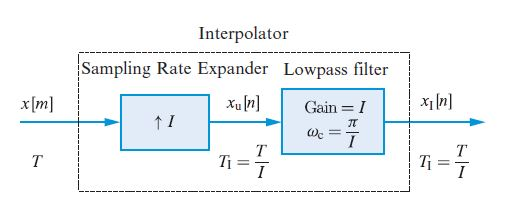
\includegraphics[width = 0.6\textwidth]{Figures/Multirate/interpolation_process}
\caption{Interpolation process: upsampling then low pass filtering \cite{DSP_DimitrisManolakis}}
\label{fig:Multirate:interpolation_process}
\end{figure}


\end{itemize}

\end{frame}

\begin{frame}[t]{Interpolation and Upsampling Recap}


\begin{figure}[ht]
\centering
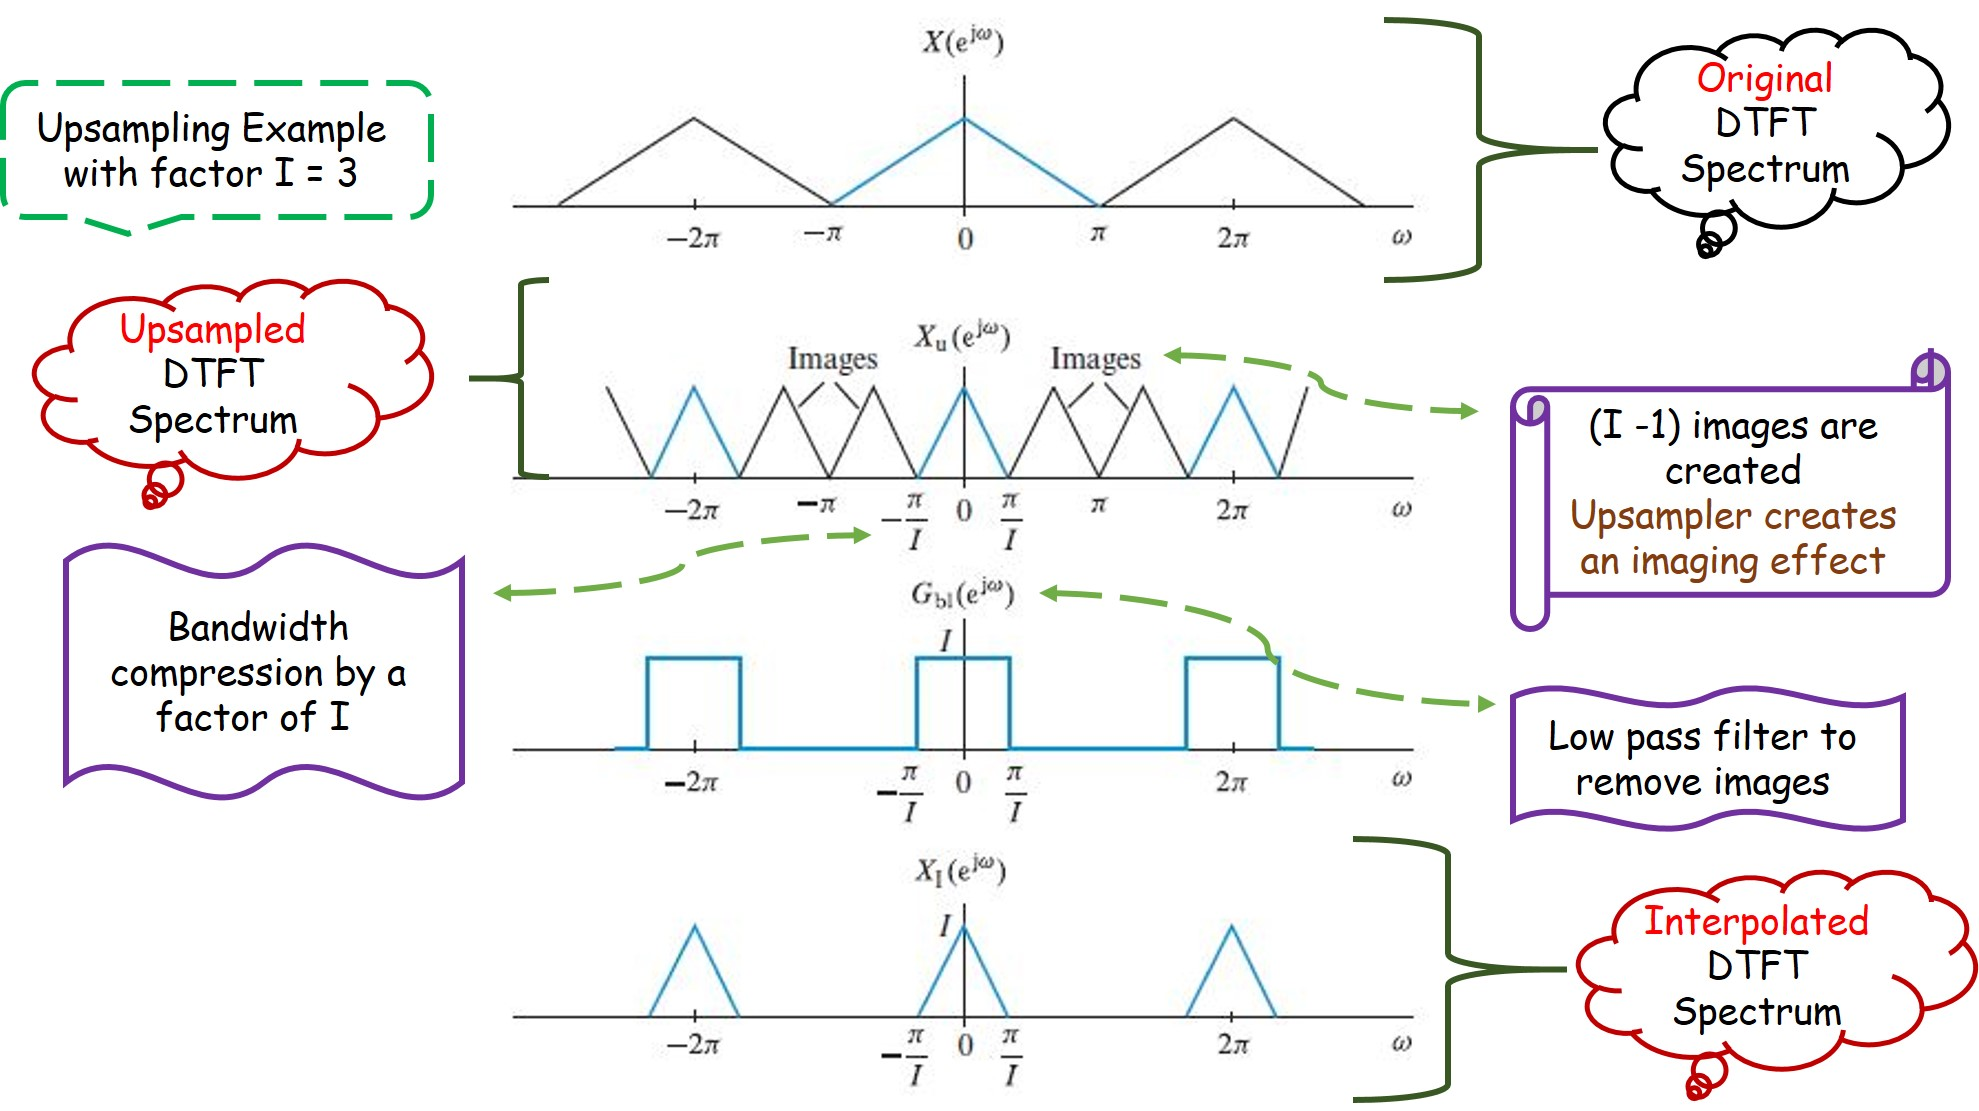
\includegraphics[width = 0.95\textwidth]{Figures/Multirate/upsampling_process}
\caption{Upsampling with a factor $I \, = \, 3$ \cite{DSP_DimitrisManolakis}}
\label{fig:Multirate:interpolation_process}
\end{figure}


\end{frame}


\subsection{Practical Upsampling}
\begin{frame}[t,allowframebreaks]{Practical Upsampling}


\end{frame}

\subsection{Resampling by non-integer factor}
\begin{frame}[t,allowframebreaks]{Resampling by non-integer factor}

\begin{itemize}

\item Sampling rate by a non-integer factor which can be expressed in the form of $T_{s_{\text{new}}} \, = \, T_{s_{\text{original}}} \, \times \, \displaystyle\frac{I}{D}$

\item Example: resample by a factor of $1.5 \, T_{s_{\text{original}}} \, = \, \displaystyle\frac{3}{2} \, T_{s_{\text{original}}}$

\item Idea: use upsampling and dowsampling together

\begin{figure}[ht]
\centering
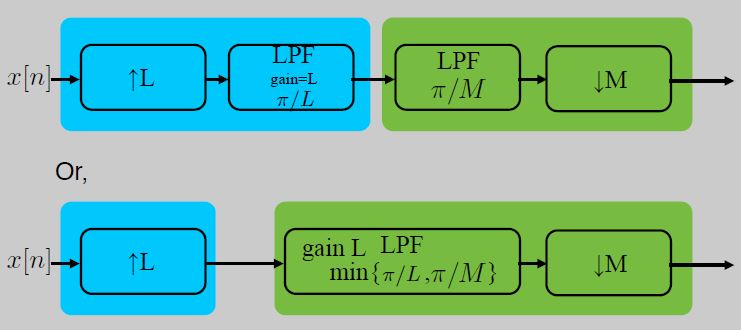
\includegraphics[width = 0.6\textwidth]{Figures/Multirate/non_integer_factor_up_and_down_sample}
\caption{Upsample and dowsample: order of operation is important}
\label{fig:Multirate:non_integer_factor_up_and_down_sample}
\end{figure}


	\begin{itemize}
	\item Can we switch order of operation ?
	
	\item No, because if we do downsample before, we loose high frequency components and won't be able to restore them in upsampling
	\end{itemize}


\end{itemize}


\end{frame}

\subsection{Polyphase Decomposition}
\begin{frame}[t,allowframebreaks]{Polyphase Decomposition: Introduction Motivation}

\begin{itemize}

\item Polyphase decomposition: decompose our filters into a sum of delayed transfer function ($z^{-k}$)  that are compressed $z^M$

\item $N$ is the length of the filter 

\item In other words, we can decompose our signals into a sum of delayed version, multiply each sample by a scalar $E_i(z)$, then add the result


\begin{figure}[ht]
\centering
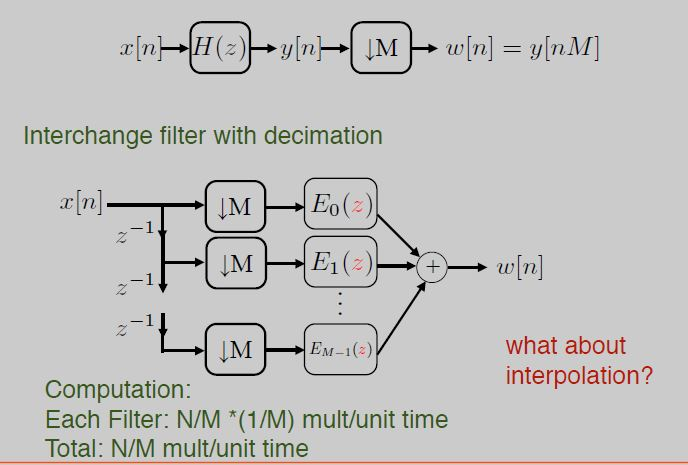
\includegraphics[scale = 0.5]{Figures/Multirate/polyphase_dowsampling}
\caption{Polyphase Structure}
\label{fig:Multirate:polyphase_dowsampling}
\end{figure}


\item Decompose our transfer function $H(z)$ into a sum of delayed transfer function which are compressed

\begin{equation}
H(z)\, = \, \displaystyle\sum_{k \, = \, 0}^{M \, - \, 1} E_k \left( \, z^M \, \right) \, z^{-k}
\end{equation}


\end{itemize}



\end{frame}


\subsection{Summary of Main Idea}


\begin{frame}[t]{Downsampling and Upsampling Ideas}

\begin{table}[!h]
\centering
	\begin{tabular}{|c|c|}
	\hline
		% header
		\multicolumn{2}{|c|}{Dowsampling}\\ \hline
		CTFT & DTFT \\ \hline
		
		Closer Images & Closer Images  \\ \hline
		
		Scaling Factor decrease & Scaling Factor decrease \\ \hline
		Bandwidth Same & Bandwidth Stretch \textcolor{blue}{but} still in $[\, - \, \pi , + \, \pi \,]$ \\ \hline		
	\end{tabular}
	\caption{Downsampling Operation Effects}
\end{table}

\end{frame}
